%Carattere dimensione 12
\documentclass[12pt,twoside]{report}

%Margini e interlinea
\usepackage[top=1in, bottom=1in, left=1.2in, right=1in]{geometry}
\pagestyle{plain}
\linespread{1.5}

%Libreria da eliminare
\usepackage{lipsum}

%Librerie utili
\usepackage[english]{babel}
\usepackage[utf8]{inputenc}
\usepackage{csquotes}
\usepackage{libertine}
\usepackage{graphicx}
\usepackage{floatflt}
\usepackage{blindtext}
\usepackage{enumitem}
\usepackage{amsthm}
\usepackage{subfig}
\usepackage{listings}
\usepackage{listingsutf8}
\usepackage{amsmath}
\usepackage{framed}
\usepackage{minibox}
\usepackage{float}
\usepackage{mathtools}
\usepackage{wrapfig}
\usepackage{longtable}
\usepackage[strict]{changepage}
\usepackage{pgfplots}
\usepackage{tikz}
\usetikzlibrary{automata,positioning}
\usepackage{amsthm}
\usepackage[
backend=biber,
style=alphabetic,
sorting=ynt
]{biblatex}
\usepackage{hyperref}
\usetikzlibrary{matrix}
\pgfplotsset{width=11cm,compat=1.9}
\usepgfplotslibrary{external}
\tikzexternalize

\hypersetup{
    colorlinks=true,
    linkcolor=blue,
    filecolor=magenta,      
    urlcolor=cyan,
    pdftitle={Membrane Systems and Petri Nets},
    pdfpagemode=FullScreen,
}

\theoremstyle{definition}
\newtheorem{definition}{Definition}[section]

\theoremstyle{fact}
\newtheorem{fact}{Fact}[section]

\addbibresource{references.bib}

\begin{document}

\title{Synchronized P System Equivalence with Petri Nets}
\author{Floris Alessandro}
\date{date}

\begin{titlepage}
\begin{figure}[t]
    \centering\includegraphics[width=0.3\textwidth]{images/logo.png}
\end{figure}
\begin{center}
    \textsc{ \LARGE{Università degli Studi di Cagliari \\}}
	\textsc{ \LARGE{Facoltà di Scienze\\ }}
	\textnormal{ \LARGE{Corso di Laurea Triennale in Informatica\\}}
	\vspace{30mm}
	\fontsize{10mm}{7mm}\selectfont 
    \textup{Synchronized P System Equivalence with Petri Nets}\\
\end{center}

\vspace{25mm}

\begin{minipage}[t]{0.47\textwidth}
	\textnormal{\large{\bf Relatore:\\}}
	{\large Prof. Giovanni Michele Pinna}
\end{minipage}\hfill\begin{minipage}[t]{0.47\textwidth}\raggedleft
	\textnormal{\large{\bf Candidato:\\}}
	{\large Floris Alessandro\\ matr. 60/61/65913}
\end{minipage}

\vspace{20mm}

\centering{\large{Anno Accademico 23/24 \\ Cagliari - 25/09/24 }}

\end{titlepage}


\include{blank-page}

\tableofcontents
\thispagestyle{empty}

\include{blank-page}

\clearpage
\pagenumbering{arabic} 

\chapter{Introduction}

In this thesis we try, successfully, to find a link between synchronized P systems and Petri nets.

P systems (known also as membrane systems) introduced in \cite{puaun2000computing}, are part of the branch of natural computing, which abstracts computing models from the architecture and the functioning of living cells.
The first models of membrane systems were starting from the single cell and its organization as a hierarchical structure of compartments, defined by membranes, where a localized biochemistry takes place.
Thus, the obtained computing device was a distributed parallel model, with multisets of objects (“chemicals") placed in regions (nodes of a tree) and processed by “reactions" of a biochemical type.
This obtained computing devices proved to be rather powerful, equivalent with Turing machines.
The model was extended in various ways, and some of this extensions are presented in ...
In this thesis we consider a class of P systems called synchronized P systems talked in \cite{aman2019synchronization},\cite{aman2022power}; this kind of synchronization works among the rules of the same membrane.
More exactly a rule synchronizing with a non-empty set of rules is applicable at least once, only if each rule from the set of rules is applicable at least once.

Petri nets are an abstract, formal model of information flow.
Introduced in \cite{petri1962kommunikation}, the major use of Petri nets is to model concurrent systems, and membrane systems can be seen as highly concurrent systems, so they can be modeled as Petri nets, and that's the object of this thesis.
From a formal point of view , Petri nets are bipartite directed graphs consisting of two kinds of nodes, called places and transitions.
Places indicate the local availability of resources, whereas transitions are actions which can occur depending on local conditions related to the availability of resources (and thus can be used to represent evolution rules associated of a membrane system).
\chapter{Background}

In this chapter we introduce some general notions as well as a more deep understanding of what P systems and Petri nets are.

\section{Basic Definitions}

\begin{definition}[Multiset]
Let $U$ be an arbitrary set. A multiset over U is a mapping \newline $m : U \rightarrow N$.
The multiplicity of an element $u$ in $m$ is given by the natural number $m(u)$.
\end{definition}

The operator $\oplus$ denotes multiset union: $m \oplus m' = m(u) + m'(u)$ for each $u$.

\begin{definition}[Alphabet]
An alphabet is a finite nonempty set of abstract symbols. Given an alphabet $V$, we denote by $V^*$
the sets of all finite strings of elements in $V$, including the empty string $\lambda$.
Every string $v \in V$ describes a multiset over $V$.
\end{definition}

\section{P Systems}

Membrane computing is a branch of natural computing, introduced by Gheorghe Paun with the definition of P systems in \cite{puaun2000computing,puaun2002membrane,paun1999computing}.

Membrane systems are based upon the notion of \textit{membrane structure}, which is a structure composed by several cell-membranes, hierarchically embedded in a main membrane called the \textit{skin membrane}.
The membranes delimit \textit{regions} and we associate with each region a set of \textit{objects}, described by some symbols over an alphabet, and a set of \textit{evolution rules}.
In the basic variant, the objects evolve according to the evolution rules, which can modify the objects to obtain new objects.
The evolution rules are applied in a maximally parallel manner: at each step, all the objects which can evolve should evolve.
If a computation \textit{halts}, so no further evolution rule can be applied, the result of the computation is defined to be the number of objects in a specified membrane.

\begin{definition}[P system]
A P system (of degree $d$, with $d \geq 1$) is a tuple
\[ \Pi = (V,\mu,w^0_1,...,w^0_d,R_1,...,R_d, i_0)\]
where:
\begin{enumerate}
  \item $V$ is an alphabet; its elements are called objects;
  \item $\mu$ is a membrane structure consisting of $d$ membranes (labeled with $1,2,...,d$);
  \item $w^0_1, 1 \leq i \leq d$, are strings from $V^*$ representing multisets over $V$ associated
  with the regions $1,2,...,d$ of $\mu$;
  \item $R_i, 1 \leq i \leq d$, are finite sets of evolution rules over $V$ associated 
  with the regions $1,2,...,d$ of $\mu$; these evolution rules are of the form $u \rightarrow v$,
  where $u$ and $v$ are strings from $V*$;
  \item $i_0$ is a number between 1 and $d$ which specifies the output membrane of %\Pi;
\end{enumerate}
A configuration of $\Pi$ is a tuple $C=(w_1,...,w_d)$ of multisets of objects, and 
$C_0=(w^0_1,...,w^0_d)$ is the initial configuration.
\end{definition}

According to \cite{agrigoroaiei2010flattening}, any P system can be flattened to a system of degree 1, we call this type of P systems \textit{flat P systems}.
For the sake of simplicity, from now on when we talk about P systems we refer to flat P systems.

\begin{definition}[Flat P system]
A flat P system is a P system of degree one
\[ \Pi = (V,\mu,w^0,R) \]

Given the fact that we're working with a one degree system we removed the subscript from $w$ and $R$. 
A configuration of $\Pi$ is a singleton $C=(w)=w$ of a multiset of objects, and 
$C_0=(w^0)=w^0$ is the initial configuration.
\end{definition}

The following example will clarify the definition of a P system.
\begin{example}
\label{ex:flat_membrane}
Consider the system of degree 1:
\begin{description}
   \item $\Pi=(V,\mu,w^0,R)$,
   \item $V=\{a,b,c\}$,
   \item $\mu=[_{1}]_{1}$,
   \item $C_0=w^0=a^2b$,
   \item $R=\{r_1:a \rightarrow b, r_2:a \rightarrow c\}$
\end{description}    
\end{example}

The system is represented in Fig 2.1.

\begin{figure}[h]
\centering

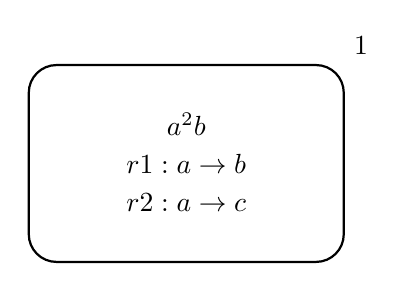
\begin{tikzpicture}
    \draw[thick, rounded corners=10pt] (0, 0) rectangle (4, 2.5) node[above right] {1};
    
    \node at (2, 1.75) {$a^2b$};
    \node at (2,1.25) (rule) {$r1: a \rightarrow b$};
    \node at (2,0.75) (rule) {$r2: a \rightarrow c$};
\end{tikzpicture}

\caption{}
\label{}
\end{figure}

The possibilities to evolve in one step from the initial configuration are: 
\begin{description}
    \item $C=w=b^3$, obtained applying $r=r_1^2$,
    \item $C=w=bc^2$, obtained applying $r=r_2^2$,
    \item $C=w=b^2c$, obtained applying $r=r_1 r_2$
\end{description}

\subsection{Synchronized P systems}

In this section we introduce a new class of P systems, P systems with \textit{synchronization among the rules of the same membrane}.
In the previous section we've seen a kind of synchronization where all regions use their rules in parallel in the maximal mode.
That synchronization that we're interested in is different, more exactly, a rule synchronizing with a non-empty set of rules is applicable at least once only if each rule from the set of rules is applicable at least once.

We call P systems with this kind of synchronization \textit{synchronized P systems}.
They are introduced and studied in \cite{aman2019synchronization,aman2022power}.

\begin{definition}[Synchronized P system]
A synchronized P system is a tuple

\[ \Pi = (V,\mu,w^0,R,\rho) \]

where:
\begin{enumerate}
    \item $(V,\mu,w^0,r)$ is a flat P system;    
    \item $\rho$ is a partial relation defined over the set $R$ of rules specifying
    the synchronization relation over the rules;
    $\rho$ is irreflexive, asymmetric and transitive;
\end{enumerate}
\end{definition}

% Questa parte è da cancellare e riscrivere 
Let's try to understand better what synchronization means:
let $(r1,r2) \in \rho$; if $r1$ is executed at least one time, then also
$r2$ has to be executed at least one time during this step, and vice versa; if that is not possible neither of them will be executed during the current step.

We use the following notation to describe an instance of $\rho$: 
$\rho=((r1 \otimes r2),(r3 \otimes r4 \otimes r5))$.
This means that $r_1$ can be executed only and only if $r_2$ can be executed at least one time;
in addition, $r_1$ it's executed at least one time only and only if also $r_2$ it's executed at least one time.

\begin{definition}[synchronization rule]
\label{def:sync_rule}
We define a synchronization rule $r_s$ as a set of rules.\\
For example $r_s=r_1 r_2 = r_1 \otimes r_2$ could be a synchronization rule.
\end{definition}

\begin{example}
    We modify \hyperref[ex:flat_membrane]{$example 1$} adding the synchronization 
    $r_1 \otimes r_2$.\\
    Now there is only one possible way to evolve in one step from the initial configuration:\\
    $C=w=b^2c$, obtained applying $r=r_1 r_2=r_1 \otimes r_2=r_{12}$;
\end{example}

In this previous example we have illustrated how the maximal parallelism behaviour is modified when synchronization of rules is used.

\section{Semantics of Synchronized P Systems}

For the purposes of this thesis, it is useful to decompose a synchronized P system computation step into multiple micro steps.
We know from \cite{busi2007causality} that the classical maximal parallelism semantics is equivalent to a causal semantics where a maximal parallelism evolution step is represented as a sequence of simple evolution steps, which are obtained by the application of a single evolution rule.
We need then to modify what a configuration is.
To represent the states of the system reached after the execution of a non maximal sequence of simple evolution rules, we introduce the notion of \textit{partial configuration} of a system.
In a partial configuration, the contents of each region is represented by two multisets.

\begin{definition}[partial configuration]
A partial configuration of $\Pi$ is a tuple $C_p=(w,w')$ 
where $w$ is the active multiset and $w'$ is the deposit (or frozen) multiset.
\end{definition}

A configuration is then a partial configuration containing no objects in the deposit;
So the initial configuration should be $C_0=(w,\emptyset)$.
Configurations represent the states reached after the execution of a maximal parallelism computation step.

Each micro step is obtained by the application of a single evolution rule.
When no evolution rule can be applied a special rule (function) will be used.

We introduce a new function, the \textit{transport function}, that transports the objects from the deposit multiset to the active multiset; this function will be used in the definition of the maximal parallelism computation step.

\begin{definition}[transport function]
Let $C=(w,w')$ be a partial configuration of $\Pi$.\newline
The transport function $transport: Conf_\Pi \rightarrow Conf_\Pi$ is defined as follows:\newline
$transport((w,w'))=(w \oplus w', \emptyset)$
\end{definition}

Using the classical maximal parallelism semantics a rule $r$ that is part of a synchronization rule $r_s$ can be executed during a computational step only if $r_s$ is executed in the same computational step.
In our causal semantics we decompose a computational step in micro steps; it results that $r$ can be executed only if $r_s$ has been executed in a previous micro step that is part of the same computational step.

\begin{definition}[computational step of causality semantics]
In our causality semantics a computational step is a sequence of evolution steps obtained by the application of a single evolution rule
\end{definition}

\section{Petri Net}

Here we define in a formal way what a Petri Net is.

\subsection{Petri Nets with Inhibitor Arcs}

Here we extend the latter definition of a Petri Net with the concept of inhibitor arcs.

\chapter{Traduction}

\section{From Basic P Systems to Petri Nets}
\label{sec:basic_p_to_pt}

To model a flat P system as a PT-net we take inspiration from \cite{kleijn2008petri}, so we introduce a separate place $(a)$ for each object $a$. 
For each evolution rule $r$ we introduce a separate transition $t^r$.
If the transformation described by a rule $r$ consumes $k$ copies of an object $a$, then we introduce a $k$-weighted arc from place $(a)$ to transition $t^r$, and similarly for molecules being produced.
Finally, assuming that, initially, the P system contains $n$ copies of object $a$, we introduce $n$ tokens into place $(a)$.
We formalise this idea as follows.

\begin{definition}[translating flat P systems into PT-nets]
\label{def:def_tr_basic}
The PT-net corresponding to $\Pi$ is:
\[ N_\Pi = (P,T,W,M_0) \]
where:
\begin{enumerate}
    \item $P=V$ and $M_0(p)=w(a)$ for every place $p=(a)$;
    \item $T$ consists of distinct transitions $t=t^r$ for every evolution rule $r \in R$;
    \item for each place $p=(a)$ the weight of the incoming arc is $W(p,t)=lhs^r(a)$ and 
    $W(t,p)=rhs^r(a)$
\end{enumerate}
\end{definition}

To capture the correspondence between the P system $\Pi$ and the PT-net $N_\Pi$, we introduce a straightforward bijection between configurations of $\Pi$ and markings of $N_\Pi$, based on the correspondence of objects and places as well as that of vector multi-rules and steps.

\begin{definition}[mapping configurations]
\label{def:map_conf}
The marking $v(C)$ corresponding to configuration $C=(w)$ is defined by $v(C)(a)=w(a)$ for every place $(a)$.   
$\beta(r_m)$, where $r_m$ is a multiset of rules over $R$, is defined by 
$\beta(r_m)(t^r)=r_m(r)$ for every transition $t^r$.  
\end{definition}

\begin{definition}[mapping vector multi-rules]
$\beta(r_m)$, where $r_m$ is a multiset of rules over $R$, is defined by 
$\beta(r_m)(t^r)=r_m(r)$ for every transition $t^r$.  
\end{definition}

\begin{fact}[]
$v(C_0)=M_0$
\end{fact}
We know that's true for the way we've defined $M_0$ in \hyperref[def:def_tr_basic]{$3.1.1$}.

\begin{fact}[]
$C \xRightarrow{r_m} C'$ if and only if $v(C)[\beta(r_m)> v(C')$ in $N_\Pi$
\end{fact}

Togheter with Fact 3.1.1, this implies that the computations of $\Pi$ coincide with step sequences of $N_\Pi$. 

\section{From Synchronized P Sytems to PTI-nets}

Here we extend the modus operandi of the section \hyperref[sec:basic_p_to_pt]{$3.1$} to translate 
a flat synchronized P system.
For each synchronizaiton rule $r_s$ (see \hyperref[def:sync_rule]{$2.2.4$}) we introduce a new transition $t^s$ (we call this syncronization transitions) and for each object $a \in V$ we introduce a new place $(a,d)$ where $d$ stands for deposit (we call this deposit places).
We keep the arcs from places $(a)$ to transitions $t^r$, but substitute the arcs from $t^r$ to $(a)$ with arcs from $t^r$ to $(a,d)$.
We then add a new place $p_{sg}$ that we call global syncronization place, and is used to check if a syncronization translation has been fired in the last step.
PT-nets are not expressive enough to model the absence of token in a place, so we need to use PT-nets extended with inhibitor arcs.
Below a more formal definition.

\begin{definition}[Translating Synchronized P systems into PTI-nets]
The PTI-net corresponding to $\Pi$ is 
\[ N_\Pi = (P,T,W,I,M_0) \]
,where:

\begin{enumerate}
  
  \item We define the set $P$ as follows:
  \begin{enumerate}
     \item for each $a \in V$, there exists a place $(a)$ and a place $(p,d)$, and 
     $M_0(p)=w(a)$ for each place $p=(a)$ and $M_0(p)=0$ for each place $p=(a,d)$;
     \item for each $r_s \in \rho$, there exists a place $(s,l)$ and a place $(s,l')$;
     $M_0(p)=1$ for each place $(s,l)$ and $M_0(p)=0$ for each place $(s,l')$
     \item exists a place $(sg)$; $M_0(p)=0$ for the place $(sg)$;
   \end{enumerate}
    
    \item $T$ consists of distinct transitions $t=t^r$ for every evolution rule $r \in R$, and 
    distinct transitions $t=t^s$ for every syncronization rule $r_s \in \rho$;
    for each $t^s$ in $T$ there exists two other control transitions $t=(t^s,1)$ and $t=(t^s,2)$;
    
    \item We define the function $W$ as follows:
    \begin{enumerate}
        \item for each place $p=(a)$, $W(p,t^r)=lhs^r(a)$, $W(p,t^s)=\sum_{r \in rs} rs(r)lhs^r(a)$, $W(t^r,p)=0$ and $W(t^s,p)=0$;
        \item for each deposit place $p=(a,d)$, $W(p,t^r)=0$ and $W(p,t^s)=0$, $W(t^r,p)=rhs^r(a)$ and $W(t^s,p)=\sum_{r \in rs} rs(r)rhs^r(a)$;
        \item for each place $p=(s,l)$, $W(p,t^s)=1$ and for each place $p=(s,l')$, $W(t^s,p)=1$;
        \item for the place $p=(sg)$, $W(t^s,p)=1$;
    \end{enumerate}

    \item We define the relation $I$ as follows:
    \begin{enumerate}
        \item for each place $p=(s,l)$, and for each transition $t^r$, where $r \in r_s$, 
        $(p,t^r) \in I$;
    \end{enumerate}
    
\end{enumerate}
\end{definition}

Once there are no more transitions that can be fired all tokens in $p=(a,d)$ are moved in the place $p=(a)$ for each $a \in V$. So exists this ghost step that indicates the end of a computation of the P system. 
\chapter{Proof of Equivalence}

In the past chapter we've modeled a flat synchronized P system as a PTI-net. 
Notice that there is not a bijection correspondence between objects in the P system and places in the net as with basic P systems.
We need a new operator.

\begin{definition}[$\psi$ operator]
We define a function $\psi: M \rightarrow M$ that takes a multiset M and returns a subset of it 
that contains only the places $p=(a)$.
\end{definition}

The definition \hyperref[def:map_conf]{$3.1.2$} remains valid.

\begin{definition}[mapping rules]
if $r_m$ has any synchronization rule we map $r_m$ with two steps:
\begin{enumerate}
    \item $\beta_1(r_m)(t^s)=r_m(r_s)$ for each $t^s$
    \item $\beta_2(r_m)(t^r)=r_m(r)$ for each $t^r$;
    $\beta_2(r_m)(t^{s'})=r_m(r_s)$ for each $t^{s'}$    
\end{enumerate}
Otherwise, if $r_m$ has no sync rules: $\beta(r_m)(t^r)=r_m(r)$ for each $t^r$
\end{definition}

\begin{fact}[]
$v(C_0)=\psi(M_{0})$
\end{fact}

\begin{fact}[]
If $r_m$ contains any sync rule: 
$C \xRightarrow{r_m} C'$ if and only if 
$v(C)[\beta_1(r_m)> v(C''') [\beta_2(r_m)>v(C'')[\gamma>v(C')$ in $N_\Pi$,
otherwise: $C \xRightarrow{r_m} C'$ if and only if 
$v(C)[\beta(r_m)>v(C'')[\gamma>v(C')$ in $N_\Pi$
\end{fact}

So we have shown that the computations of $\Pi$ coincide with $n$ step sequences of $N_\Pi$ with $n=1$ or $n=2$, 
\chapter{Proof of Equivalence}

We now want to prove that a computational step of $\Pi$ is equivalent (coincide) to a computational step of $N_\Pi$.
To do so, we need to demonstrate that both systems produce the same result under the same conditions. 
Recall that the result of a computation of a synchronized P system $\Pi$ is a configuration $C=(w1,\emptyset)$, and the result of a computation of a PTI-net $N_\Pi$ is a marking $\psi(M)$.

To demonstrate the correspondence between the two models of computation let's introduce a bijection between configurations of $\Pi$ and markings of $N_\Pi$.

\begin{definition}[Mapping configuration]
    Let $C=(w1,w2)$ be a configuration of $\Pi$.\newline
    Then the corresponding marking $v(C)$ of $N_\Pi$ is defined by:
    \[ v(C)(a)=w_1(a) \text{ and } v(C)(a,d)=w_2(a)\]
    for each place $(a)$ and for each place $(a,d)$
\end{definition}

Follows the fact:
\begin{fact}[]
$v(C_0)=\psi(M_0)$
\end{fact}

Now we define a correspondence between micro steps of $\Pi$ and steps of $N_\Pi$ using inference rules.

\noindent
\begin{tabular}{ @{} r c l @{} }
  
  R1. & \infer{
  M_1 \xrightarrow{t_s} M_2
  }
  {\text{$\Pi$ executes $C_1 \xrightarrow{r_s} C_2$}} \\ \\

  R2. & \infer{
   M_1 \xrightarrow{t^r t^{s'}} M_2
  }
  {\text{$\Pi$ executes $C_1 \xrightarrow{r} C_2$ and $\exists t^s \in \mathcal{T}_{n-1}$}} \\ \\
  
  R3. & \infer{
   M_1 \xrightarrow{t^r} M_2
  }
  {\text{$\Pi$ executes $C_1 \xrightarrow{r} C_2$ and not exists a $t^s \in \mathcal{T}_{n-1}$}} \\ \\

  R4. & \infer{
   M_1 \xrightarrow{\gamma t^{s'}} M_2
  }
  {\text{$\Pi$ executes $C_1 \xrightarrow{\delta} C_2$ and $\exists t^s \in \mathcal{T}_{n-1}$}} \\ \\

  R4. & \infer{
   M_1 \xrightarrow{\gamma} M_2
  }
  {\text{$\Pi$ executes $C_1 \xrightarrow{\delta} C_2$ and not exists a $t^s \in \mathcal{T}_{n-1}$}} \\ \\
\end{tabular}

\printbibliography[heading=bibintoc, title={References}]
\addcontentsline{toc}{chapter}{Acknowledgments}
\chapter*{Acknowledgments}
Grazie a tutti.

\end{document}